\subsection{Evolution of the computation time through games}
Tweaking the settings of MCTS or minimax could in theory allow to reach equivalent results as minimax but these would not be achieved using the same computation time.
This section explores this idea by comparing the evolution of this time for both algorithms.

As Monte Carlo Tree Search simulates a game to its end at each iteration it is reasonable to think that the computation
time of each move will decrease during the game.
As the end approaches, the number of moves to simulate decreases.
Minimax on the other hand should use a more uniform time during the game since it is a simple tree exploration up to a certain depth (with pruning which will on average offer a constant improvement)
It could be interesting to see if the time of MCTS ends up better than the one of minimax, and if so around which turn it happens.
This could allow to use both algorithms at their best.

Figure~\ref{fig:benchmark-time_turn} shows this evolution.
One can notice that as expected the compution time of MCTS decreases with time, by a factor of almost four from the beginning to the end of the game.
Most of this evolution happens in the first twenty-five moves. 
However, minimax times are so low (for similar final results) that mcts never reaches them. 
Improvements in the implementation could change this as mentioned in section~\ref{sec:param_approach}.

\begin{figure}[ht]
    \centering
    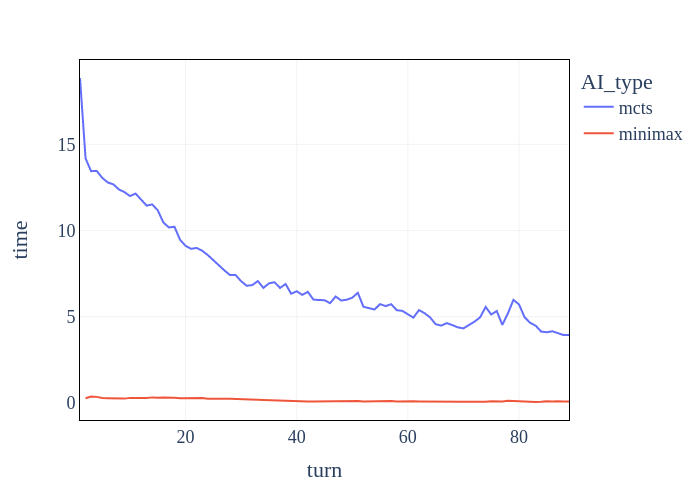
\includegraphics[width=\linewidth]{plots/AvgTime_n20000.png}
    \caption{Computing time [s] of both used algorithms (MCTS with $n=20k$) as a function of the number of turn played. MCTS diminishes but does not reach minimax in these settings. The dataset consists in about 80 games with $n=20k$ and 8 different parameters of $p$. However, as $p$ doesn't play a role in the execution time (as shown on figure \ref{fig:benchmark-p_bplot}), we can consider that the 80 games are indeed comparable in their execution times.}
    \label{fig:benchmark-time_turn}
\end{figure}